\chapter{Week 8}
\section{Neural Network Autoregression}
\begin{figure}[!htbp]
    \centering
    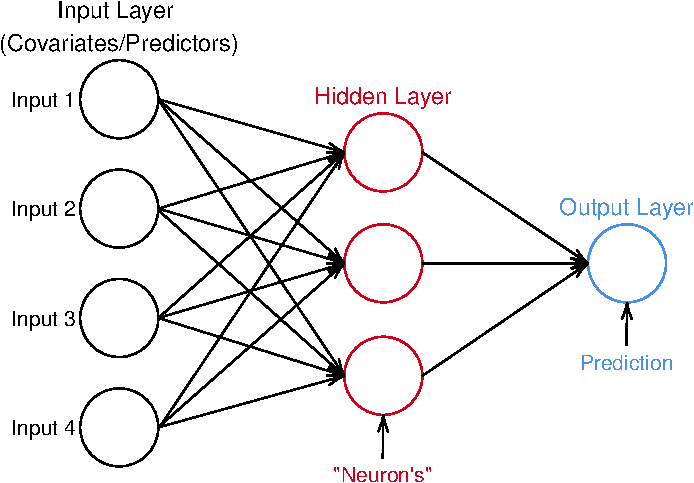
\includegraphics[width=0.75\textwidth]{8_1-neural.pdf}
    \caption{Simple Neural Network ``Architecture''}
\end{figure}
It's possible to have several hidden layers and multiple
neurons in each hidden layer.

Any particular layer in the neural network regression,
the inputs are mapped to the neurons in the hidden layer using
a simple linear transformation: inputs
are mapped to the $ j^{\text{th}} $ neuron linearly. The value taken on the $ j^{\text{th}} $
neuron is
\[ z_j=b_j+\sum_{i=1}^{4} w_{ij}x_{i} \]
where $ b_j $ is a function, $ x_i $ is the $ i^{\text{th}} $ input, and $ w_{ij} $
are the weights.

To calculate the inputs to the next layer, a non-linear transformation
is applied. For example, using the sigmoid function:
\[ S(z)=\frac{1}{1+e^{-z}} \]
The final model is a complex non-linear function of the inputs.

\subsection*{Neural Network AR}
\begin{itemize}
    \item Input layer: $ X_t,\ldots,X_{t-p} $.
    \item Output layer: $ X_{t+1} $.
\end{itemize}
A neural network model with $ k $ hidden states (assuming one hidden layer)
we call a $ \NNAR{p,k} $ model.
\begin{Remark}{}{}
    If $ k=0 $, then $ \NNAR{p}=\AR{p} $. The inputs are mapped
    linearly to the outputs.
\end{Remark}
\subsection*{Seasonal Neural Network AR}
\begin{itemize}
    \item Input layer: $ X_{t},\ldots,X_{t-p},X_{t-m},X_{t-P_m} $
          where $ m $ is the seasonal lag.
    \item Output layer: $ X_{t+1} $.
\end{itemize}
We call this a $ \NNSAR{p,k,P}{m} $ model.

The model selection of choosing $ k $, $ p $, and $ P $
can be carried out using cross-validation where the weights are estimated using ordinary
least squares.

\subsection*{Prediction Intervals}
If $ \symbf{X}_t=(X_t,\ldots,X_{t-p},X_{t-m},\ldots,X_{t-P_m})^\top $
denotes the vector of predictors, then we can posit an additive stochastic model for
$ X_{t+1} $ as
\[ X_{t+1}=f(\symbf{X}_t)+\varepsilon_{t+1} \]
where $ f $ is the neural network.

By calculating the residuals
$ \hat{\varepsilon}_t=X_t-\hat{f}(\symbf{X}_t) $,
prediction intervals can be estimated using the bootstrap
\[ X_{T+1}^{(b)}=\hat{f}(\symbf{X}_T)+\hat{\varepsilon}_{T+1}^{(b)}\quad(b=1,\ldots,B) \]
We can then construct a prediction interval by using
the empirical quantiles from the simulated distribution of the
forecast $ 1 $-step ahead. This process can be iterated multiple
times to produce forecasts as well as prediction intervals for
forecasts at longer time horizons.

\href{https://github.com/Hextical/university-notes/blob/master/year-3/semester-2/STAT 443/code/8.1 - Neural Network Autoregression.R}{[R Code] Neural Network Autoregression}
\section{Comparing Various Forecasting Methods}
\begin{itemize}
    \item \href{https://github.com/Hextical/university-notes/blob/master/year-3/semester-2/STAT 443/code/8.2 - Comparing Various Forecasting Methods.R}{[R Code] Comparing Various Forecasting Methods}
    \item The M3-Competition: Results, Conclusions and Implications
\end{itemize}
\section{Conditional Heteroscedasticity}
\[ \Uunderbracket{\text{Hetero}}_{\text{different}}\text{-}\Uunderbracket{\text{scedasticity}}_{\text{variance}} \]
\[ \Uunderbracket{\text{Hetero}}_{\text{same}}\text{-}\Uunderbracket{\text{scedasticity}}_{\text{variance}} \]
\begin{Example}{}{}
    If $ X_t $ is weakly stationary, then $ X_t $ is ``homoscedastic''
    in the sense that $ \Var{X_t}=\sigma_X^2 $ does not change over time.
\end{Example}
\begin{Definition}{Heteroscedastic}{}
    We say a time series $ X_t $ is \textbf{heteroscedastic}
    if $ \Var{X_t}=\sigma_{X,t}^2 $; that is, the variance
    depends on $ t $ and changes at some points.
\end{Definition}
\begin{Remark}{}{}
    Heteroscedastic time series are \underline{not} stationary.
\end{Remark}
Asset price data terminology: In the context of conditionally
heteroscedastic time series, we often consider asset price or ``financial''
time series. Suppose $ X_t= $ price of an asset at time $ t $.
\begin{Definition}{Returns, Log-returns}{}
    If $ X_t $ is the value of an asset at time $ t $, then
    the \textbf{return} (relative gain) $ Y_t $ of the
    asset at time $ t $ is
    \[ Y_t=X_t-X_{t-1}=\nabla X_t \]
    Furthermore, the \textbf{log-returns}
    of a positive asset price series $ X_t $
    are
    \[ Y_t=\log*{\frac{X_t}{X_{t-1}}}=\log{X_t}-\log{X_{t-1}} \]
\end{Definition}
\begin{Remark}{}{}
    ``Volatility'' $ \iff $ ``Variance''.
\end{Remark}
\href{https://github.com/Hextical/university-notes/blob/master/year-3/semester-2/STAT 443/code/8.3 - ARCH and GARCH Introduction.R}{[R Code] ARCH and GARCH Introduction}

A common observation, especially prominent with financial and asset
price data, is that periods of volatility or heteroscedastic
tend to cluster.

Why? Big ``shocks'' cause volatile periods, that further propagate
volatility until things ``calm down.''

ARMA and linear time series models are not useful for capturing this phenomenon
as we will see in the next example.
\begin{Example}{}{}
    Let $ X_t \sim \AR{1} $; that is, $ X_t=\phi X_{t-1}+W_t $ where $ \abs{\phi}<1 $.
    \[ \E{X_t\given X_{t-1},X_{t-2},\ldots}=\phi X_{t-1} \]
    ARMA models ``model'' the conditional mean $ X_{t-1},X_{t-2},\ldots $.
    \[ \Var{X_t\given X_{t-1},X_{t-2},\ldots}=\sigma_W^2 \]
    $ X_{t-1},X_{t-2},\ldots $ leave the variance untouched.
\end{Example}
\begin{Definition}{Conditionally heteroscedastic}{}
    We say a time series $ X_t $ is \textbf{conditionally heteroscedastic}
    if
    \[ \Var{X_t\given X_{t-1},X_{t-2},\ldots}=\sigma_{X,t}^2 \]
    that is, the variance changes with $ t $.
\end{Definition}
It's possible to have a time series $ X_t $ that's
homoscedastic, but is also conditionally heteroscedastic.

\section{ARCH and GARCH Models}
\begin{Definition}{Autoregressive conditionally heteroscedastic (ARCH)}{}
    Let $ W_t $ be a unit variance strong white noise; that is,
    $ \E{W_t}=0 $ and $ \Var{W_t}=1 $. We say $ X_t $
    follows an \textbf{autoregressive conditionally heteroscedastic}
    (ARCH) model if there exists parameters $ \omega> 0 $, $ \alpha_1\ge 0 $
    such that $ X_t=\sigma_t W_t $ where
    \[ \sigma_t^2=\omega+\alpha_1 X_{t-1}^2 \]
    where $ \sigma_t^2 $ is the conditional variance and $ W_t $
    is a white noise.
\end{Definition}
\begin{Remark}{}{}
    ARCH is from Robert Engle, 1982.
\end{Remark}
\begin{Definition}{Autoregressive conditionally heteroscedastic $ [\ARCH{p}] $}{}
    We say $ X_t $ follows an \textbf{autoregressive conditionally heteroscedastic} model
    of order $ p $, if $ W_t $ is a strong white noise with $ \E{W_t^2}=1 $
    and
    \[ X_t=\sigma_t W_t \]
    \[ \sigma_t^2=\omega+\sum_{j=1}^{p} \alpha_j X_{t-j}^2 \]
    where $ p>0 $, $ \omega>0$, and $\alpha_j\ge 0$ for $j=1,\ldots,p$.
    We write $ X_t \sim \ARCH{p} $.
\end{Definition}
\begin{Remark}{}{}
    \begin{enumerate}[(1)]
        \item $ \sigma_t^2 $ is called the ``conditional variance'' or ``volatility.''
              Imagine that there exist a representation $ X_t=g(W_t,\ldots,W_{t-1}) $
              (stationary process satisfying the ARCH model). Then, for example, in the
              $ \ARCH{1} $ case,
              \[ \sigma_t^2=\omega+\alpha_1 X_{t-1}^2=g_\sigma(W_{t-1}W_{t-2},\ldots) \]
              Therefore,
              \[ \Var{X_t\given W_{t-1},W_{t-2},\ldots}=\Var{\sigma_t W_t\given W_{t-1},\ldots}=\sigma_t^2\Var{W_t}=\sigma_t^2 \]
              $ \Var{W_t}=1 $ identifies $ \sigma_t^2 $ as conditional variance.
        \item Engle won the Nobel Prize in economics in part for ``methods of analyzing economic
              time series with time varying volatility (ARCH)'' in 2003.
        \item One problem noted early on was that $ \ARCH{p} $
              models required large orders of $ p $ to model asset returns
              which suggested \emph{generalizing} the model.
    \end{enumerate}
\end{Remark}
\begin{Definition}{Generalized autoregressive conditional heteroskedasticity (GARCH)}{}
    We say $ X_t $ follows a \textbf{generalized autoregressive conditional heteroskedasticity}
    (GARCH) model
    if $ W_t $ is unit variance strong white noise and
    \[ X_t=\sigma_t W_t \]
    \[ \sigma_t^2=\omega+\sum_{j=1}^{p} \alpha_j X_{t-j}^2+\sum_{k=1}^{q} \beta_k \sigma_{t-k}^2 \]
    where $ q\ge 0 $, $ p>0 $, $ \omega>0 $, $ \alpha_j\ge 0 $ for $ j=1,\ldots,p $, and
    $ \beta_k\ge 0 $ for $ k=1,\ldots,q $.
    We write $ X_t \sim \GARCH{p,q} $.
\end{Definition}
\begin{Remark}{}{}
    The $ \GARCH{p,q} $ model was proposed by Bollerslev (1986).
\end{Remark}
\begin{Remark}{}{}
    \begin{itemize}
        \item $ \GARCH{p,0}\equiv \ARCH{p} $.
        \item $ \GARCH{0,0} $ is a white noise.
    \end{itemize}
\end{Remark}
\begin{Proposition}{Properties of GARCH}{}
    Suppose for the moment that there exists ``a stationary and causal time
    series $ X_t $ satisfying the $ \GARCH{p,q} $ model,''
    $ X_t=g(W_t,W_{t-1},\ldots)\implies \sigma_t^2=g_\sigma(W_{t-1},W_{t-2},\ldots) $,
    then
    \begin{enumerate}[(1)]
        \item $ \E{X_t}=\E{\sigma_t}\E{W_t}=0 $ since $ \sigma_t $ and $ W_t $ are
              independent.
              \[ \gamma_X(h)=\E{X_{t+h}X_t}=\E{\sigma_{t+h}W_{t+h}\sigma_t W_t}=0 \]
              since $ W_{t+h} $ is independent of the rest.
              Therefore,
              GARCH series have mean zero and are serially uncorrelated by construction.
        \item Suppose $ X_t \sim \ARCH{1} $.
              \begin{align*}
                  X_t^2
                   & =\sigma_t^2 W_{t}^2                             \\
                   & =\sigma_t^2(W_t^2+1-1)                          \\
                   & =\sigma_t^2+(W_t^2-1)                           \\
                   & =\omega+\alpha_1 X_{t-1}^2 +\sigma_t^2(W_t^2-1)
              \end{align*}
              Now, note that $ \sigma_t^2=g(W_{t-1},W_{t-2},\ldots) $,
              and $ W_t^2-1 $ is a mean zero random variable. Hence,
              the \textbf{last} term is a weak white noise.

              Therefore, $ X_t^2 \sim \AR{1} $ process (weak white noise innovations).
        \item In general, if $ X_t \sim \GARCH{p,q} $, then $ X_t^2 $
              follows an ARMA model with weak white noise innovations.
              \[ X_t \sim \GARCH{p,q}\implies X_t^2\text{ is serially correlated (ARMA).} \]
    \end{enumerate}
\end{Proposition}
\href{https://github.com/Hextical/university-notes/blob/master/year-3/semester-2/STAT 443/code/8.4 - ARCH and GARCH Update.R}{[R Code] ARCH and GARCH Models}
\section{Stationarity of GARCH Models}
Suppose $ X_t \sim \GARCH{p,q} $ model.

\underline{Question}: Under what conditions on $ \omega,\alpha_1,\ldots,\alpha_p,
    \beta_1,\ldots,\beta_p $, does a stationary process $ \set{X_t}_{t\in\mathbf{Z}} $
satisfy these questions?

\begin{Remark}{}{}
    Suppose a stationary solution exists that is a causal Bernoulli shift; that is,
    \[ X_t=g(W_t,W_{t-1},\ldots) \implies \sigma_t^2=g_\sigma(W_{t-1},W_{t-2},\ldots) \]
    If $ \Var{X_t}<\infty $, note
    \[ \Var{X_\sigma}=\Var{\sigma_t W_t}=\E{\sigma_t^2 W_t^2}=\E{\sigma_t^2}=\sigma_X^2 \]
    Using the GARCH recursion:
    \[ \E{\sigma_t^2}=\omega+\sum_{j=1}^{p} \alpha_j \E{X_{t-j}^2}+\sum_{k=1}^{q} \beta_k \E{\sigma^2_{t-k}} \]
    \[ \implies\sigma_X^2=\omega+\sum_{j=1}^{p} \alpha_j \sigma_X^2 +\sum_{k=1}^{q}\beta_k \sigma^2_X  \]
    Solving gives
    \[ \sigma_X^2=\frac{\omega}{1-\sum_{j=1}^{p} \alpha_j-\sum_{k=1}^{q} \beta_k}  \]
    Suggests that in order for a solution to exist in $ L^2 $, we need at least
    \[ \sum_{j=1}^{p} \alpha_j + \sum_{k=1}^{q} \beta_k <1 \]
    (Bollerslev, 1986)
\end{Remark}
Consider $ \GARCH{1,1} $ case; that is,
\[ X_t=\sigma_t W_t \]
\[ \sigma_t^2=\omega+\alpha X_{t-1}^2+\beta \sigma_{t-1}^2 \]
In order to get a stationary solution for $ X_t $ that satisfies
$ X_t=\sigma_t W_t $, we need a stationary casual variance process.

Let $ f(z)=\alpha z^2+\beta $.
Iterate GARCH recursion:
\begin{align*}
    \sigma_t^2
     & =\omega+\alpha X_{t-1}^2+\beta \sigma_{t-1}^2                                                                          \\
     & =\omega+\alpha(\sigma_{t-1}^2 W_{t-1}^2)+\beta \sigma_{t-1}^2                                                          \\
     & =\omega+(\alpha W_{t-1}^2+\beta)\sigma_{t-1}^2                                                                         \\
     & =\omega+f(W_{t-1})(\omega+\alpha X_{t-2}^2+\beta \sigma_{t-2}^2)                                                       \\
     & =\omega+\omega f(W_{t-1})+f(W_{t-1})(\alpha X_{t-2}^2+\beta \sigma_{t-2}^2)                                            \\
     & =\omega+\omega f(W_{t-1})+\omega f(W_{t-1})f(W_{t-2})+f(W_{t-1})f(W_{t-2})(\alpha X_{t-3}^2+\beta_{t-3}\sigma_{t-3}^2) \\
     & \vdotswithin{=}                                                                                                        \\
     & =\omega\biggl(1+\sum_{i=1}^{\infty} \prod_{j=1}^i f(W_{t-j})\biggr)                                                    \\
     & =g_\sigma (W_{t-1},W_{t-2},\ldots)
\end{align*}
Posit solution
\[ \sigma_t^2=\omega\biggl(1+\sum_{j=1}^{\infty} \prod_{i=1}^j f(W_{t-i})\biggr) \]
\underline{Question}: When is this series well-defined?
\[ \prod_{i=1}^j f(W_{t-i})=\expon[\bigg]{\sum_{i=1}^{j} \log*{f(W_{t-j})}} \]
Now, note that $ \sum_{i=1}^{j} \log*{f(W_{t-j})} $ is a random walk. Therefore,
\[ \sum_{i=1}^{j} \log*{f(W_{t-j})}\to
    \begin{cases*}
        +\infty                                               & with probability $ 1 $ if $ \E*{\log*{f(W_0)}}>0 $ \\
        -\infty                                               & with probability $ 1 $ if $ \E*{\log*{f(W_0)}}<0 $ \\
        \text{oscillates between $ -\infty $ and $ +\infty $} & if $\E*{\log*{f(W_0)}}=0$
    \end{cases*} \]
The good case is when $ \E*{\log*{f(W_0)}}<0 $, and it causes the terms to tend to zero fast.
\begin{Theorem}{}{}
    A stationary solution $ X_t $ exists to the $ \GARCH{1,1} $ equations if and only if
    \[ \gamma=\E[\big]{\log{\alpha W_0^2+\beta}}<0\quad\text{[Top Lyapunov Exponent]} \]
    The solution is of the form
    \[ X_t=\sigma_t W_t \]
    \[ \sigma_t^2=\omega\biggl(1+\sum_{j=1}^{\infty} \prod_{i=1}^j (\alpha W_{t-j}^2+\beta)\biggr)=
        g(W_{t-1},W_{t-2},\ldots) \]
    where $ g $ is a function that is not linear; that is, we have a non-linear time series.
\end{Theorem}
\begin{Remark}{}{rem_garch11}
    \begin{enumerate}[(1)]
        \item If $ \gamma<0 $, $ \omega=0 $ forces $ X_t\equiv 0 $. Therefore, we will
              normally assume $ \omega>0 $.
        \item The condition $ \gamma=\E[\big]{\log{\alpha W_0^2+\beta}}<0 $ depends
              on the distribution of $ W_t $.
        \item A sufficient condition is $ \alpha_1+\beta_1<1 $.
    \end{enumerate}
\end{Remark}
\begin{Proof}{\Cref{remark:rem_garch11} (3)}{}
    Jensen's Inequality: If $ f:\mathbf{R}\to\mathbf{R} $ is convex, then
    \[ f\bigl(\E{X}\bigr)\le \E[\big]{f(X)} \]
    and the opposite holds if $ f $ is concave. We note that $ \log{x} $
    is concave, hence
    \[ \E[\big]{\log{\alpha W_0^2+\beta}}\le \log*{\E{\alpha W_0^2+\beta}}=\log{\alpha+\beta}<0 \]
    only when $ \alpha+\beta<1 $.
\end{Proof}
\begin{Remark}{Second-order Stationarity of $ \GARCH{1,1} $ Equation}{}
    If $ \alpha_1+\beta_1>1 $, we have seen that $ \Var{X_t} $ is not well-defined.
    If $ \alpha_1+\beta_1<1 $, then
    \[ \E{\sigma_t^2}=\E*{\frac{\omega}{1-\alpha-\beta}}<\infty \]
    Assuming $ \alpha_1+\beta_1<1 $, then we know a stationary solution exists and
    in this case, $ X_t $ is weakly stationary and is a weak white noise.
    \[ \gamma_X(h)=\E{X_{t+h}X_t}=\E{\sigma_{t+h}W_{t+h}\sigma_t W_t}=0 \]
\end{Remark}
\begin{figure}[!htbp]
    \centering
    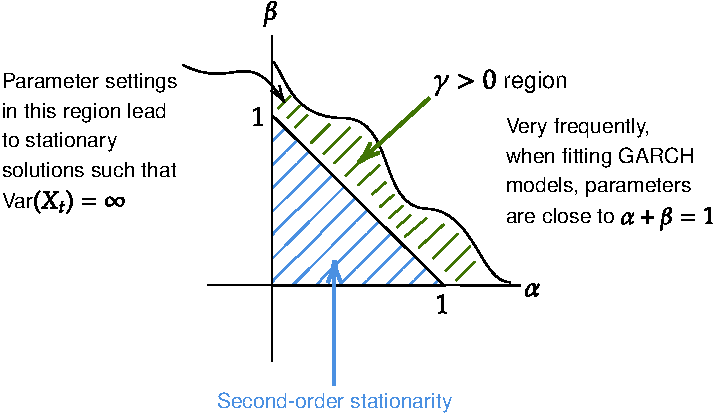
\includegraphics[width=0.75\textwidth]{8_5_Stationarity.pdf}
    \caption{$ \GARCH{1,1} $ ``Region of Stationarity''}
\end{figure}
\section{\texorpdfstring{$ \dagger $}{†} Stationarity of General \texorpdfstring{$ \GARCH{p,q} $}{GARCH(𝑝, 𝑞)}}
General conditions exist for when a $ \GARCH{p,q} $ process has a strictly stationary solution: Let
\begin{align*}
    \tau_{t} & =(\beta_{1}+\alpha_{1} W_{t}^{2}, \beta_{2}, \ldots, \beta_{q-1})\in \mathbf{R}^{q-1}                  \\
    \xi_{t}  & =(X_{t}^{2}, 0, \ldots, 0) \in \mathbf{R}^{q-1}                                                        \\
    \alpha   & =(\alpha_{2}, \ldots, \alpha_{p-1}) \in \mathbf{R}^{p-2}                                               \\
    I_{c}    & =c\times c \text{ identity matrix.}                                                                    \\
    N        & =(\omega, 0, \ldots, 0) \in \mathbf{R}^{p+q-1}                                                         \\
    Y_{t}    & =(\sigma_{t}^{2}, \ldots, \sigma_{t-q+1}^{2}, X_{t}^{2}, \ldots, X_{t-p+1}^{2}) \in \mathbf{R}^{p+q-1} \\
    M_{t}    & =\begin{bmatrix}
        \tau_{t} & \beta_{q} & \alpha  & \alpha_{p} \\
        I_{q-1}  & 0         & 0       & 0          \\
        \xi_{t}  & 0         & 0       & 0          \\
        0        & 0         & I_{p-2} & 0
    \end{bmatrix}\in \mathbf{R}^{(p+q-1) \times (p+q-1)}
\end{align*}

\begin{Theorem}{}{}
    $X_{t}$ solves the $ \GARCH{p,q} $ equations if and only if
    \[
        Y_{t}=M_{t} Y_{t-1}+N
    \]
    This representation is known as the Markov representation of the GARCH equations.
    This defines a first order vector autoregression for $Y_{t}$ with
    (random) matrix coefficients $M_{t}$.
\end{Theorem}
Let $A_{t}$ be a stationary sequence of random $(p+q-1) \times (p+q-1)$ matrices, and define,
for an arbitrary norm on matrices $\norm{}$ the scalar random variables.
\[ r_{t}=\norm{A_{t} A_{t-1} \ldots A_{1}} \]
under some relatively mild conditions (ergodicity)
\[ \gamma=\lim\limits_{{t} \to {\infty}}\biggl[\frac{1}{t} \E[\big]{\log{r_{t}}}\biggr] \]
is well-defined and is called the top Lyapunov exponent of the sequence
$A_{t}$ for $t \in \mathbf{Z}$.
This result is coming from Ergodic theory in the 1970s.
\begin{Theorem}{}{}
    A stationary solution to the $ \GARCH{p,q} $ equations exists if and only if
    \[ \gamma<0 \]
    where $\gamma$ is the top Lyapunov exponent of sequence
    $M_{t}$ for $t \in \mathbb{Z}$ appearing in the Markov representation.
    When a stationary solution exists, it is causal and unique.
\end{Theorem}
\begin{Theorem}{Theorem 1 of Bollerslev (1986)}{thm_1_bollerslev_1986}
    A necessary and sufficient condition for there to exist a second order stationary
    solution to the $ \GARCH{p,q} $ equations is that
    \[ \sum_{j=1}^{p} \alpha_{j}+\sum_{\ell=1}^{q} \beta_{\ell}<1 \]
\end{Theorem}

\section{Identifying GARCH Models}
The decision to fit a volatility (GARCH) model to a time series often
arises from
\begin{enumerate}[(1)]
    \item Observing volatility (conditional heteroskedasticity)
          in a series.
    \item Conditional variance forecasting is of specific interest
          (e.g., risk analysis, financial TS analysis).
\end{enumerate}
If strong serial correlation is observed in the series, one
often fits initially an ARMA model, and then
fits a GARCH model to the residuals.
\subsection*{Identifying Serial Correlation}
Recall that the normal ACF bounds (blue lines)
are constructed based on the assumption that
the series is a \emph{strong} white noise. A GARCH
model is a \emph{weak} white noise.

\subsection*{ACF Bounds for Weak White Noise}
Suppose for example that $ X_t \sim \GARCH{1,1} $, then
\[ \gamma_X(h)=0\quad(h\ge 1) \]
\[ \hat{\gamma}_X(h)\approx \frac{1}{T} \sum_{j=1}^{T-h} X_t X_{t+h}\implies \E{\hat{\gamma}_X(h)}=0 \]
\begin{align*}
    \Var*{\sqrt{T}\hat{\gamma}_X(h)}
     & =\frac{1}{T} \sum_{j=1}^{T-h} \sum_{k=1}^{T-h} \E{X_{j}X_{j+h}X_{k}X_{k+h}}                                            \\
     & =\frac{1}{T} \sum_{j=1}^{T-h} \sum_{k=1}^{T-h} \E{\sigma_j W_j \sigma_{j+h}W_{j+h}\sigma_{k+h}W_{k+h}\sigma_k W_{k+h}} \\
     & =\frac{1}{T} \sum_{j=1}^{T-h} \E{X_{j+h}^2 X_j^2}                                                                      \\
     & \approx \E{X_0^2 X_{-h}^2}
\end{align*}
\begin{itemize}
    \item If $ j>k $, then $ W_{j+h} $ is independent of the other terms.
    \item If $ k>j $, then $ W_{k+h} $ is independent of the other terms.
    \item $ \E{X_j+h^2 X_j^2} $ does not simplify to a product $ \sigma_X^4 $ since
          $ X_{j+h}^2 $ is correlated with $ X_j^2 $.
\end{itemize}
\begin{Theorem}{}{}
    If $ X_t $ is a weak white noise (suitably weakly dependent), then
    \[ \sqrt{T}\hat{\gamma}_X(h)\xrightarrow[T\to\infty]{D}\N[\big]{0,\E{X_0 X_{-h}^2}} \]
\end{Theorem}
\begin{Remark}{}{}
    \begin{enumerate}[(1)]
        \item $ \E{X_0^2 X_{-h}^2} $ can be consistently estimated from the sample:
              \[ \hat{\sigma}_h^2=\frac{1}{T} \sum_{j=1}^{T-h} X_{j+h}^2 X_j^2 \]
              Therefore, an approximate $ (1-\alpha) $ prediction interval for $ \hat{\rho}(h) $
              under the assumption of a weak white noise is
              \[ \pm \frac{1}{\sqrt{T}}z_{1-\alpha/2}\frac{\hat{\sigma}_h}{\hat{\gamma}(0)} \]
              The blue line depends on $ h $ due to $ \hat{\sigma}_h $.
        \item Note that
              \[ \E{X_0^2 X_{-h}^2}=\bigl(\E{X_0^2}\bigr)^2+\Uunderbracket{\Cov{X_0^2,X_{-h}^2}}_{\text{GARCH}\implies \Cov{\cdot}>0} \]
              Hence, in a GARCH setting, the weak white noise intervals for ACF are (often) larger.
    \end{enumerate}
\end{Remark}
\href{https://github.com/Hextical/university-notes/blob/master/year-3/semester-2/STAT 443/code/8.7 - Identifying GARCH models.R}{[R Code] Identifying GARCH Models}
